%\section{Bayesian regression}
\chapter{Bayesian Optimization}
Whereas traditional regression workflow is the following: From data, fit model parameters, make predictions using the parameters. 
The Bayesian framework allows us to skip the dependency of a single set of parameters and instead use all sets of parameters 
by treating the set of parameters as a random quantity, $\theta$. What is of interest is the predictive posterior distribution,  
\begin{align}\label{Predictive2}
    p(y|x, \mathcal{D})
\end{align}
Before bringing the parameters/unknown quantities into play, 
we can ask: What quantities can we play with? This question is answered in two different ways in Gaussian process regression
and Bayesian Neural network regression.

\section{Discriminative model as surrogate model}
Discriminative modeling
$$p(y|x)$$

\section{Using a generative model as surrogate model}
Given a generative model over $x$ and $y$ paramitised with $\theta$, we are dealing with the joint distribution
$$p(x,y|\theta)$$
and we are interested in the condtional distribution of y given x, 
$$p(y|x, \theta_{y|x})$$
where we have put subscript on $\theta$ in order to jump up a level of abstraction since, 
in fact there is just a mapping between them $\theta_{y|x} := g(\theta, y, x)$ 

% $$\alpha p(y|x) + (1-\alpha) \mathcal{N}(0,1)$$

% so what should $\alpha$ be? Here we can find inspiration from a Poission point process. 


\begin{align*}
    p(y|x, \mathcal{D}) &= \int p(y|x,\theta_{y|x})p(\theta_{y|x}|\mathcal{D}) d\theta_{y|x}  \\
    &=  p(y|x,\hat \theta_{y|x})
\end{align*}
Where the last equation holds as we assume that $p(\theta_{y|x}|\mathcal{D})$ is a delta function
i.e. a point estimate with value $\hat \theta_{y|x}$. In the case of our Gaussian mixture model, 
we obtain a point estiamte from the EM algorithm for the variance $\Sigma_{y|k}$, mean value $\mu_{y|k}$ and proportion $\pi_{y|k}$
for each component $k = 1,2, \dots, K$
$$\hat \theta_{y|x} = (\hat\Sigma_{y|k}, \hat\mu_{y|k}, \hat\pi_{y|k})_{k=1}^K$$

However, we are not satisfied with the variance estimate for the regression, as it is way too small for areas with
no observed data. It is therefore necessary to manipulate the variance estimate accoring to that observation. 
We multiply the variance obtained using expectation-maximization on the joint distribution with the
inverse of the probability of the data $x$, and control that the scaling factor is not going wild!

$$\hat\Sigma_{y|k} =\Sigma_{y|k}^{GMM} \frac{1}{\max(p(x), 0.01)}$$

In a way this is a manipulation in a Bayesian spirit, as we let prior and subjective knowledge influence the
varience prediction. 



\subsection{Inclusion of prior distribution}
The conditional distribution $p(y|x)$ is without a prior. Therefore
its beliefs is not really ok.. In the flavour of a Poission point process, 
we introduce the prior.. 
$$p_{bayes}(y|x) = \frac{p(x)\cdot N \cdot p(y|x) + \lambda p_{prior}(y)}{Z}$$
where the normalization constant $Z$ makes sure the manipulated density integrates
to 1, i.e. 
$$Z =\int p(x)\cdot N \cdot p(y|x) + \lambda p_{prior}(y) dy =p(x)\cdot N+\lambda $$


\begin{figure}[H]
    \centering
    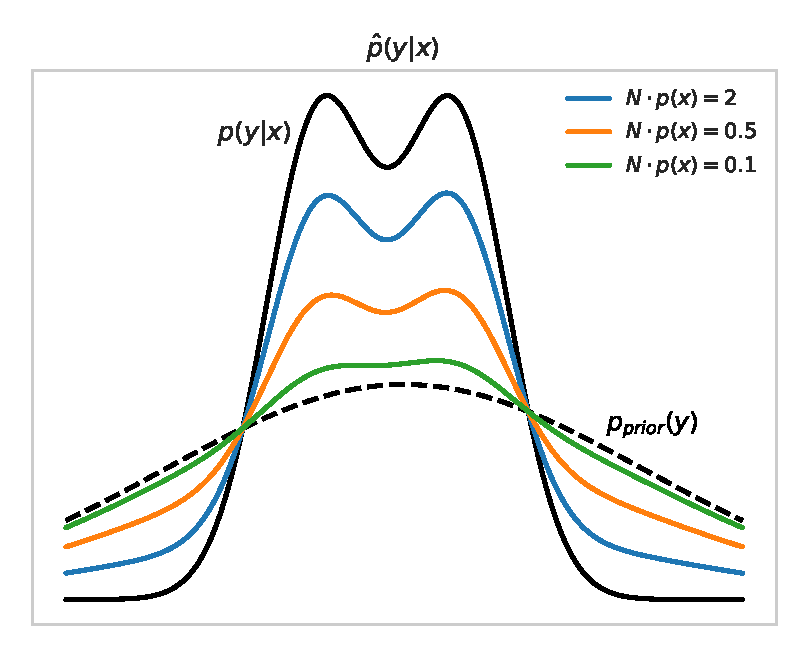
\includegraphics[]{Pictures/mixture_predictive_bayesian.eps}
\end{figure}

\begin{figure}[H]
    \centering
    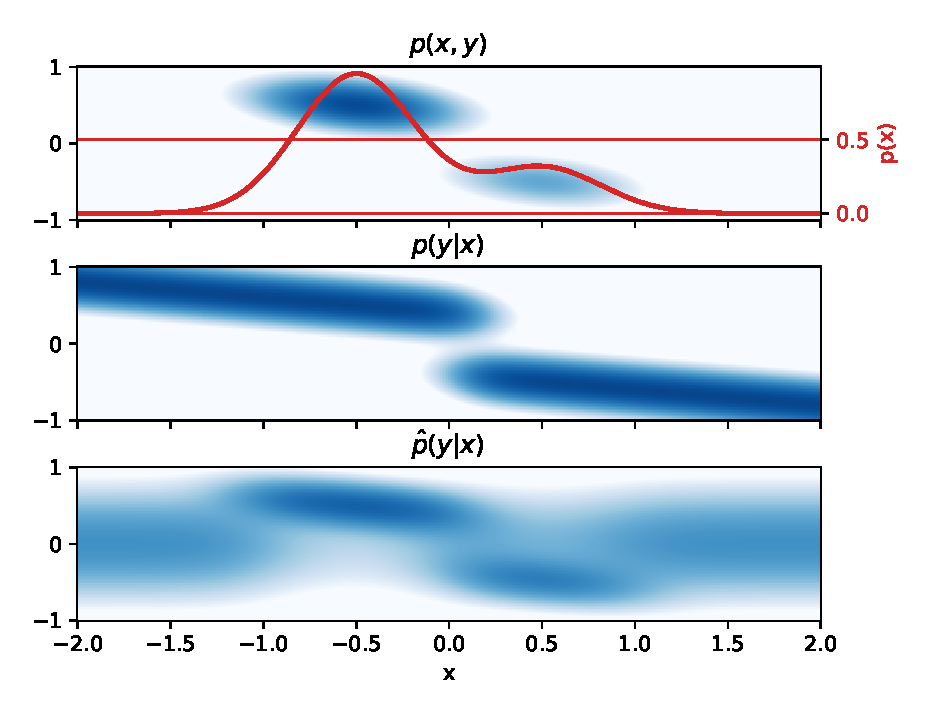
\includegraphics[]{Pictures/mixture_predictive_bayesian2D.eps}
\end{figure}


\subsubsection*{mean of $p_{bayes}(y|x)$}
\begin{align*}
    E_{p_{bayes}(y|x)}[y] &= \int y \cdot \frac{f(n,p(x)) \cdot p(y|x) + \lambda p_{prior}(y)}{Z} dy\\
    &= \left(p(x)\cdot N \cdot E_{p(y|x)}[y] + \lambda \cdot E_{p_{prior}(y)}[y] \right) \frac{1}{Z}\\
    &= \frac{p(x)\cdot N\cdot E_{p(y|x)}[y]}{p(x)\cdot N+\lambda}
\end{align*}

\subsubsection*{variance of $p_{bayes}(y|x)$}
We first calculate the second moment, 
\begin{align*}
    E_{p_{bayes}(y|x)}[y^2] &= \int y^2 \cdot \frac{p(x)\cdot N \cdot p(y|x) + \lambda p_{prior}(y)}{Z} dy\\
    &= (p(x)\cdot N\cdot E_{p(y|x)}[y^2] + \lambda E_{p_{prior}(y)}[y^2] ) \frac{1}{Z}\\
    &= \frac{p(x)\cdot N \cdot(Var_{p(y|x)}[y]+E_{p(y|x)}[y]^2) + \lambda Var_{p_{prior}(y)}[y]}{p(x)\cdot N+\lambda}
\end{align*}

So the variance is calculated as, 
$$V_{p_{bayes}(y|x)}[y] = E_{p_{bayes}(y|x)}[y^2] - E_{p(x,y)}[y]^2$$

\subsubsection*{implementation}
It is not necessary to calculate the conditional distribution, since, using Bayes rule
$$p(y|x) = \frac{p(x,y)}{p(x)}$$
so gives
$$p_{bayes}(y|x) = \frac{p(x)\cdot N \cdot p(y|x) + \lambda p_{prior}(y)}{Z} = \frac{N \cdot p(x,y) + \lambda p_{prior}(y)}{Z}$$


$$E_{p(x,y)}[y] = \int_y \int_x yp(x,y) dx dy = \int_y y p(y) dy = E_{p(y)}[y]$$

\section{Acquisition function}
A popular choice of acquisition function is expected improvement:
\begin{align*}
    \mathbb{E}_{y_*|\textbf{x}_*,D_n}[\min(0,y_{\min}-y_*)] &= ??\\
    \mathbb{E}[\min(0,y_{\min}-y_*)|\textbf{x}_*,D_n] &= \int_{-\infty}^\infty \min(0,y_{\min}-y_*) p(y_*|\textbf{x}_*,D_n) dy_*\\
    &= \int_{-\infty}^{y_{\min}} (y_{\min}-y_*) p(y_*|\textbf{x}_*,D_n) dy_*\\
    &\approx \frac{1}{N} \sum_{\theta \in \Omega } [y_{\min}-f_\theta(x)],
\end{align*}

where $\Omega = \{\theta|f_{\theta}(x)< y_{\min}\}$

%\section{uncertainties}
%Alatoric vs epistemic uncertainties 